% Crucial Preamble
\documentclass[12pt,letterpaper]{article} \usepackage{amsmath} \usepackage{graphicx} \usepackage[margin=1in]{geometry} \usepackage{longtable}  \usepackage{amssymb}

% Extra Preamble
\usepackage{fancyhdr} \usepackage{enumitem} \usepackage{float} \usepackage{soul}
\usepackage{multicol} \usepackage[compact]{titlesec}


% frames with display breaks
\usepackage{mdframed}
\allowdisplaybreaks

% change spacing
\usepackage{setspace}
\setlength{\parskip}{0.4\baselineskip}

% Remove paragraph indentation
\setlength{\parindent}{0pt}

% Reduce space before and after section headings
%\titlespacing*{\section}{0pt}{0.1\baselineskip}{0.2\baselineskip}

% changes font
%\renewcommand{\familydefault}{\sfdefault}

% adds header and footer
\pagestyle{fancy}
\fancyhead{} \fancyhead[C]{MAT 2322 Cheat Sheet} \fancyhead[L]{MAT2322} \fancyhead[R]{Owen Daigle}
\fancyfoot{} \fancyfoot[C]{\thepage}


\begin{document}
	
	\begin{center}
		\Large\textbf{MAT 2322 Cheat Sheet} \\
		\vspace{0.5em}
	\end{center}
	
	\section{Curves [L1, L2]}
	A curve takes in a scalar and gives a vector. We say:
	\begin{equation*}
		r(t)=\left<f(t),g(t),h(t)\right>
	\end{equation*}

	We can break up any 3d situation into its components. 
	
	\begin{mdframed}[]
		\textbf{Ex. } Find the limit as t approaches infinity of $r(t)=\left<\sin t, \cos t, t^2\right>$
	
	We will just take the limit of each of the 3 dimensions. 
	\begin{align*}
		\lim_{t\to\infty} \sin t = 0 \qquad \lim_{t\to\infty} \cos t = 1 \qquad \lim_{t\to\infty} t^2 = 0 \\
    	\text{So, we know that the limit is } \left<0,1,0\right>
	\end{align*}
	\end{mdframed}

	\begin{mdframed}[]
		\textbf{Ex. } Find the arc length of: $r(t) = \left<\cos t, \sin t, t\right>$ from 0 to $2\pi$
		
		We know that the arc length is just: $L = \int_a^{b} |r'(t)|dt$.
		
		So we will find the derivative of each dimension, then take the square root of the squares of each dimension, then we integrate from 0 to $2\pi$.
	\end{mdframed}
	
	\section{Multi Variable Differentiation [L2, L3]}
	We define the Gradient Vector of $f$ as $\nabla f$, and the Direcional Derivitive of $f$ on direction $u$ (where $u$ is a unit vector) as $D_u f$.
	\begin{align*}
		\nabla f = \left<\frac{df}{dx},\frac{df}{dy}\right> \\
		D_u f(x,y) = \nabla f \cdot u
	\end{align*}

	We can extend this to the next dimension by just adding a third value to each of those formulas ($\frac{df}{dz}$ and $z$).
	
	\begin{mdframed}[]
		\textbf{Ex. } Find the directional derivative of $f(x,y) = x^2y^3 - 4y$ in the durection of $v=\left<2,5\right>$ at $(2,1)$.
		
		We need to get the gradient vector, and the unit vector $u$. 
		\begin{align*}
			u = \frac{v}{|v|}=\frac{v}{\sqrt{2^2+5^2}}=\frac{v}{\sqrt{29}}=\left<\frac{2}{\sqrt{29}},\frac{5}{\sqrt{29}}\right>
		\end{align*}
	
		Then we need to get the gradient vector at $(2,1)$.
		\begin{align*}
			\nabla f(2,1)=\left<2xy^3,3x^2y^2-4\right> = \left<-4,8\right>
		\end{align*}
	
		Now we just plug into the Directional Derivitive formula. We use the dot product to calculate.
		\begin{align*}
			D_u f(x,y) = \nabla f \cdot u = \left<-4,8\right> \cdot \left<\frac{2}{\sqrt{29}},\frac{5}{\sqrt{29}}\right> = CALC
		\end{align*}
	\end{mdframed}

	The tangent plane equation is:
	\begin{align*}
		T= F_x (x_0, y_0) (x-x_0) + F_y (x_0, y_0) (y-y_0)
	\end{align*}
	Where $x_0$, $y_0$ is the point we want to find the tangent plane at, and $x, y \in \mathbb{R}$. We can extend this to more dimensions as well.
	
	\section{Max/Min [L3, L4]}
	If a point is a local max/min, then all first order partial derivitives at that point are 0. 
	
	Critical points are points where all first order partial derivitives are 0. These are not necissarily max/mins.
	
	We have the discriminant of $D = \left| 
	\begin{array}{cc}
		f_{xx} & f_{xy} \\
		f_{xy} & f_{yy}
	\end{array} \right|$
	We say that if:
	\begin{itemize}[]
		\item $D>0$ and $f_{xx} > 0$ then $f(a,b)$ is a local min
		\item $D>0$ and $f_{xx} < 0$ then $f(a,b)$ is a local max
		\item $D<0$ then $f(a,b)$ is a saddle point
		\item $D=0$ then we don't know anything
	\end{itemize}

	\begin{mdframed}[]
		\textbf{Ex.} Find the extreme values of $x^4 + y^4 - 4xy + 1$.
		
		We start by finding the first order derivatives and get:
		\begin{align*}
			f_x = 4x^3 - 4y \qquad f_y = 4y^3 - 4x
		\end{align*}
		Then setting them equal to 0, we have 2 equations and 2 unknowns.
		\begin{align*}
			4x^3 - 4y = 0 = 4y^3 - 4x \quad \implies \quad x=0, x=\pm 1 \quad \implies \quad (1,1), (0,0), (-1,-1)
		\end{align*}
		Now we have 3 crit points. We will find the discriminant at each of those points. To do this, we need the second order derivatives.
		\begin{align*}
			f_{xx} = 12x^2 \qquad f_{yy} = 12y^2 \qquad f_{xy} = f_{yx} = -4
		\end{align*}
		Now subbing into the discriminant equation of $D = \left| 
		\begin{array}{cc}
			f_{xx} & f_{xy} \\
			f_{xy} & f_{yy}
		\end{array} \right|$ at each point, we get:
		\begin{itemize}[noitemsep]
			\item (0,0): $D<0$: Saddle Point
			\item (1,1): $D>0$: Min/Max
			\item (-1,-1): $D>0$: Min/Max
		\end{itemize}
		Now we need to find if it is actually a min or max by looking at $f_{xx}$.
		\begin{align*}
			f_{xx}(1,1) = 12 > 0\\
			f_{xx}(-1,-1) = 12>0
		\end{align*}
		So they are both local mins.
	\end{mdframed}
	
	\section{Lagrange Multipliers [L5, L6]}
	If we need to find the max and min of a function $f$ in a constraint $g$, we use lagrange multiplyers. 
	\begin{align*}
		\nabla f = \lambda \nabla g
	\end{align*}

	When working with these zones, we need to test the critical points, and also all the points on the bounds of the constraint. 
	
	We know how to find the critical points (first partial derivitive to 0) but for the points on the bounds, we need to use lagrange multipliers, solve for lambda, and then solve for those points. 
	\begin{figure}[H]
		\centering
		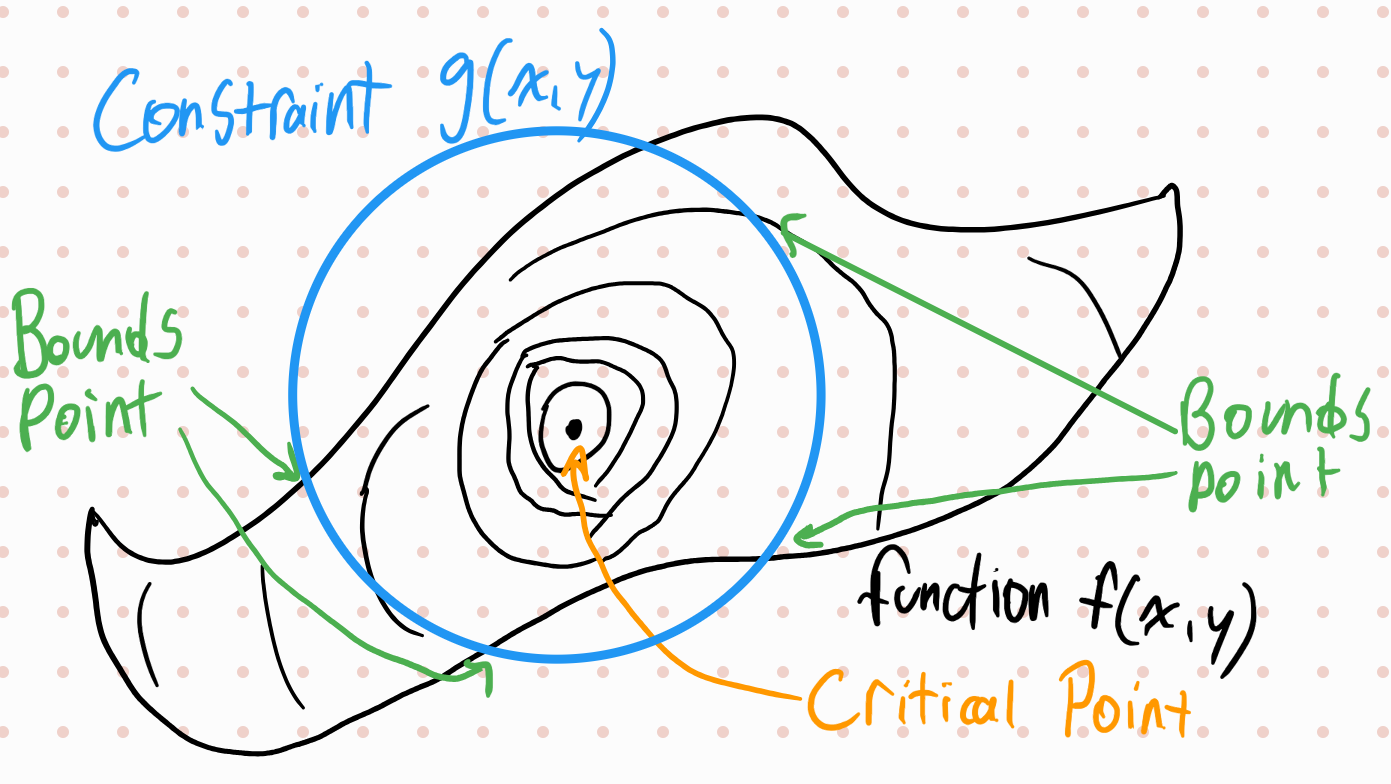
\includegraphics[width=0.5\linewidth]{lagrange.png}
	\end{figure}

	\begin{mdframed}[]
		\textbf{Ex. } Find the maximum and minimums of $f(x,y) = x^2+y^2 +4x-4y$ on $x^2+y^2\le 9$.
		
		We start by finding the crit points by setting $f_x=f_y=0$.
		\begin{align*}
			2x+4=0 \implies x=-2 \qquad 2y-4 = 0 \implies y=2
		\end{align*}
		We have a point $(0,0)$.
		
		Now we need to use lagrange multiplyers. 
		\begin{align*}
			& 2x+4 = \lambda 2x \implies \lambda = \frac{2x+4}{2x} \qquad 2y-4 = \lambda 2y \implies \lambda = \frac{2y-4}{2y}\\
			& \frac{2y-4}{2y} = \frac{2x+4}{2x} \qquad \implies \qquad x=-y
		\end{align*}
		Now subbing this into the constraint, we get:
		\begin{align*}
			y^2 + y^2 = 9 \implies y=\frac{\pm 3}{\sqrt{2}}
		\end{align*}
		Since we know that $x=-y$, we have 2 more points of: $\left(\frac{3}{\sqrt{2}},\frac{-3}{\sqrt{2}}\right)$, $\left(\frac{-3}{\sqrt{2}},\frac{3}{\sqrt{2}}\right)$
		
		Then we can take those 3 points, check which one is the min/max, and we are done.
	\end{mdframed}

	We can also do lagrange multipliers using 2 constraints.
	\begin{align*}
		\nabla f = \lambda \nabla g + \mu \nabla h
	\end{align*}
	
	\section{Double Integrals}
	This is just 2 integrals put together. We just solve the first one first, and then the second one. 
	
	\subsection{Double Integrals in Rectangular Regions [L6, L7]}
	It is easy to integrate a rectangular region of $R = [a,b] \times [c,d]$ by doing:
	\begin{align*}
		V = \int^b_a \int^d_c f(x,y) dxdy
	\end{align*}
	We can also change the order of integration and do the dx first or dy first (ensure to also change the bounds if changing the order).
	
	We just solve the first integral, and then solve the second integral using the result from the first integral.
	\begin{mdframed}[]
		\textbf{Ex. } Find the volume of $\int_R \int x-3y^2 dA$ on $R=[0,2]\times [1,2]$.
		
		We just add the x bounds (0,2) and y bounds (1,2) to the integral and solve to get:
		\begin{align*}
			\int^2_0 \int_1^2 x-3y^2 dydx = \int_0^2 x-7 dy = -12
		\end{align*}
	\end{mdframed}
	
	\subsection{Double Integrals in General Regions [L8]}
	This is very similar to double integrals in rectangular regions except that $dxdy \ne dydx$.
	
	To determine whether to do dxdy or dydx, we check if it is a type 1 or type 2 integral.
	
	For a type 1 integral, (functions are horizontal) we do:
	\begin{figure}[H]
		\centering
		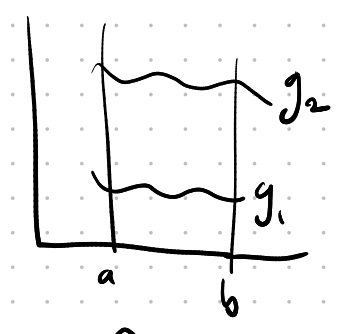
\includegraphics[width=0.3\linewidth]{type1.png}
	\end{figure}
	\begin{align*}
		\int_a^b \int^{g_2}_{g_1} f(x,y) dydx
	\end{align*}

	For a type 2 integral (functions are vertical) , we do:
	\begin{figure}[H]
		\centering
		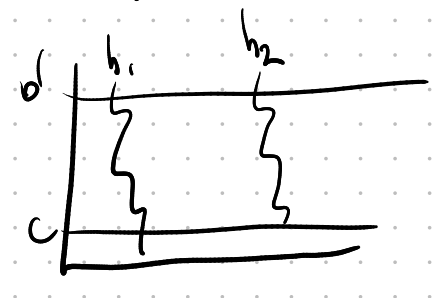
\includegraphics[width=0.3\linewidth]{type2.png}
	\end{figure}
	\begin{align*}
		\int_a^b \int_{h_1}^{h_2} f(x,y) dxdy
	\end{align*}
	
	\subsection{Polar Coordinates [L8, L9, L10]}
	When we are working with polar coordinates, rather than using the x and y, we use r and $\theta$ where r is the radius, and $\theta$ is the angle from the positive x axis. 
	
	To convert from cartesian to polar, we use:
	\begin{align*}
		x = r\cos(\theta) \qquad y = r\sin(\theta)\\
		\int_R \int f(x,y) dA = \int^{\beta} _{\alpha} \int^b_a f(r\cos\theta,r\sin\theta)\cdot r\cdot drd\theta
	\end{align*}
	
	\begin{mdframed}[]
		\textbf{Ex. } Find the shaded area:
		\begin{figure}[H]
			\centering
			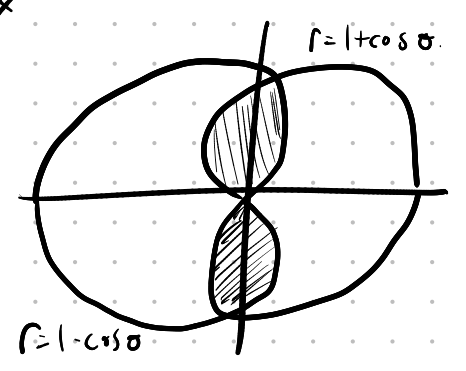
\includegraphics[width=0.4\linewidth]{figure.png}
		\end{figure}
	
		We are not sure how to do this using cartesian coordinates. It looks simple with polar though.
		
		We see that the radius at any point on the top half is just 0 to the function $1+\cos\theta$. The angle goes through the whole $2\pi$ but we will just do half of that, and then double the integral. It goes from $-\pi/2$ to $\pi/2$.
		\begin{align*}
			2\cdot \int^{\frac{\pi}{2}}_\frac{-\pi}{2} \int_0^{1+\cos\theta} r\cdot drd\theta = SOLVE
		\end{align*}
	\end{mdframed}

	
	\section{Applications of Double Integrals [L11]}
	
	We analyse 4 applications in this course.
	
	\subsection{Charge}
	We are given the charge density $\sigma (x,y)$ on a domain $D$ and we can calculate it by simply integrating the sigma function.
	
	\begin{mdframed}[]
	\textbf{Ex. } The triangular region bounded by $y=1-x, y=1, x=1$ has charge density $\sigma=xy$. Find the charge density.
	
	The only real hard part is finding the bounds for the integral that we will use. 
	
	We can draw out the area and get:
	\begin{center}
		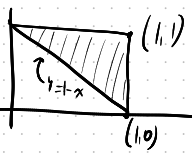
\includegraphics[width=0.2\linewidth]{ex}
	\end{center}
	Now we can see that if we start integrating vertically, at any point we go from $1-x$ to 1. Then if we do the horizontal part, we go from 0 to 1.
	\begin{align*}
		\int^1_0\int^1_{1-x} xy dxdy = \int^1_0 \left(2x^2-x^3\right) dy = \frac{5}{24}
	\end{align*}
	
	\end{mdframed}
	
	\subsection{Finding Mass from Density}
	Generally we are given a density function $\rho (x,y)$ and we need to find the mass of a domain $D$ from that, we use the following integral:
	\begin{align*}
		m = \iint\limits_D \rho(x,y) dA
	\end{align*}
	
	\subsection{Finding center of mass}
	To find this, we need to know the moment equations using the density $\rho$ on the domain $D$.
	\begin{align*}
		M_x = \iint\limits_D y\rho(x,y) da \qquad M_y = \iint\limits_D x\rho(x,y)
	\end{align*}
	Then we can get the center of mass:
	\begin{align*}
		\overline{x} = \frac{M_y}{m} \qquad \overline{y} = \frac{M_x}{m}
	\end{align*}

	\begin{mdframed}[]
	\textbf{Ex. } Find the center of mass of a triangular region with vertices (0,0), (1,0), (0,2) with $\rho (x,y) = 1+3x+y$
	
	Like always, the hardest part is finding the correct bounds for the integral.
	
	Here we need to draw the triangle where we get:
	\begin{center}
		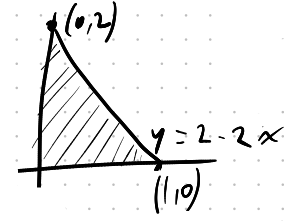
\includegraphics[width=0.2\linewidth]{ex2}
	\end{center}
	The line is just gotten by calculating the slope between the 2 points. 
	
	Firstly we need the mass:
	\begin{align*}
		0\ge y \ge 2-2x \qquad 0\ge x\ge 1\\
		m = \int _0^1 \int^{2-2x}_0 \left(1+3x+y\right) dydx = ... = \frac{8}{3}
	\end{align*}
	Now we have the mass, so we can then find the center of mass using their respective equations.
	
	\begin{align*}
		\overline{x}= \frac{M_y}{m} = \frac{\int^1_0 \int^{2-2x}_0 x (1+3x+y) dydx}{8/3} = \frac{3}{8} \int^1_0 \int^{2-2x}_0 \left(x+3x^2 +xy\right) dydx = ... = \frac{8}{3} \\
		\overline{y} = \frac{M_x}{m} = \frac{\int^1_0 \int^{2-2x}_0 y (1+3x+y) dydx}{8/3} = \frac{3}{8} \int^1_0 \int^{2-2x}_0 \left(y+3xy +y^2\right) dydx = ... = \frac{11}{16}	
	\end{align*}
	
	\end{mdframed}
	
	\subsection{Inertia}
	This is very similar to the center of mass:
	\begin{align*}
		I_x = \iint\limits_D y^2 \rho(x,y) dA \qquad I_y = \iint\limits_D x^2 \rho(x,y)dA \qquad I = \iint\limits_D \left(x^2 + y^2 \right) \rho(x,y) dA
	\end{align*}
	It is just a case of finding the correct bounds of the integrals (using the domain given) and then simply solving the integral.
	
	
	\section{Surface Area [L12]}
	The surface area of a function $f$ on a domain $D$ 	can be calculated as:
	\begin{align*}
		A(s) =  \iint\limits_D \sqrt{\left(\frac{\partial f}{\partial x} \right)^2 + \left(\frac{\partial f}{\partial y}\right)^2 + 1} dA
	\end{align*}

	\begin{mdframed}[]
	\textbf{Ex. } Find the surface area of $f(x,y)=x^2+y^2$ in $D={(x,y) | x^2+y^2\le 9}$.
	
	We know the domain, which looks like we can use polar coordinates with a radius of 3, and angle of 0 to $2\pi$. 
	
	Using the surface area formula, we need the partial derivatives. 
	\begin{align*}
		\frac{\partial f}{\partial x} = 2x \qquad \frac{\partial f}{\partial y} = 2y
	\end{align*}	
	Now I can just sub into the equation and convert to polar coordinates. 
	\begin{align*}
		A(s) = \iint \limits_D \sqrt{(2x)^2 + (2y)^2 + 1} dA = \int_0^{2\pi} \int^3_0 \sqrt{\left(4r^2\left(\cos^2 (\theta) + \sin^2(\theta)\right)+1\right)}r \cdot drd\theta \\= ...=\frac{\pi}{6} (37\sqrt{37}-1)
	\end{align*}
	
	\end{mdframed}

	\section{Change of Variables [L13]}
	Whenever we perform a transformation on a function (such as rectangular coordinates to polar coordinates), we need to multiply by a factor known as the \textbf{Jacobian}
	
	Recall that with the polar coordinates, we had to always multiply by a factor of $r$, this is because of the Jacobian.
	\begin{align*}
		J = \frac{\partial (x,y) }{\partial (u,v)} = \left|\begin{array}{cc} \frac{\partial x}{\partial u} & \frac{\partial x}{\partial v} \\ \frac{\partial y}{\partial u} & \frac{\partial y}{\partial v} \end{array}\right|
	\end{align*}
	Note that the matrix in this equation is the determinant.
	
	\begin{mdframed}[]
	\textbf{Ex. } Find the jacobian for the polar coordinates ($x=r\cos\theta, y=r\sin\theta$).
	
	We need to find the 4 partial derivatives. 
	\begin{align*}
		J = \frac{\partial (x,y) }{\partial (r,\theta)} = \left|\begin{array}{cc} \frac{\partial x}{\partial r} & \frac{\partial x}{\partial \theta} \\ \frac{\partial y}{\partial r} & \frac{\partial y}{\partial \theta} \end{array}\right| = \left|\begin{array}{cc} \cos\theta & -r\sin\theta \\ \sin\theta & r\cos\theta \end{array}\right| = r\cos^2\theta - (-r\sin^2\theta) = r
	\end{align*}
	And we know this is true since we always add the $r$ factor when converting to polar.
	\end{mdframed}
	
	\section{Triple Integrals [L14]}
	Just like double integrals, if we are integrating over a rectangular area, then the bounds are interchangeable. This does not apply over a general area.
	
	We have 3 types of triple integrals:
	
	\begin{figure}[H]
		\centering
		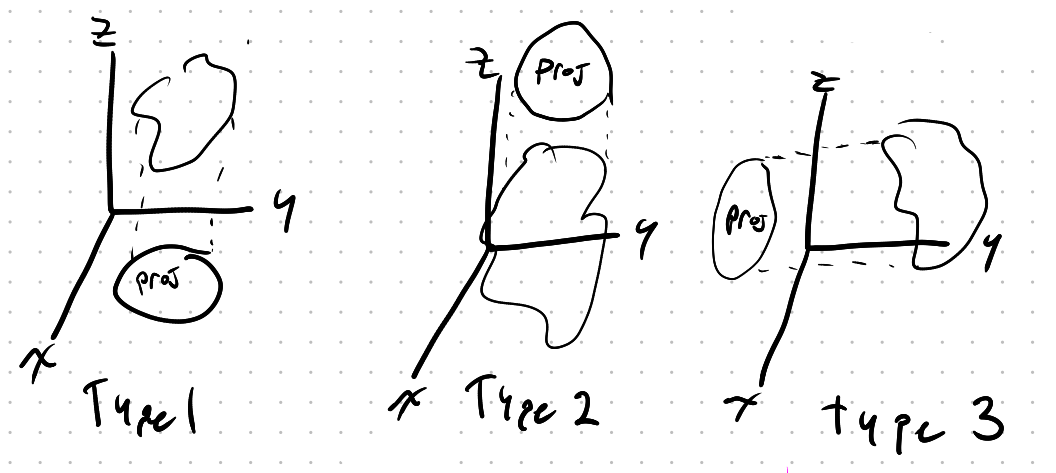
\includegraphics[width=0.7\linewidth]{screenshot001}
	\end{figure}
	
	\subsection{Triple Integrals in Cylindrical Coordinates [L15, L16]}
	In cylindrical coordinates, we convert $(x,y,z) \to (r,\theta, z)$ where:
	\begin{align*}
		x = r\cdot \cos(\theta) \qquad y = r\cdot \sin(\theta) \qquad z = z
	\end{align*}
	Then we have the jacobian of $J=r$.
	
	We can use logic to reason that $r =\sqrt{x^2+y^2}$, and $\theta = \arctan\left(\frac{x}{y}\right)$.
	
	\begin{mdframed}[]
	\textbf{Ex.} We have a cylindrical shell that is 20m tall, with inner radius 6m, and outer radius 7m. Write the inequalities we would use for the integral.
	
	This is a very simple question. 
	
	We know that z goes from \textit{0 to 20}. 
	
	the radius is just the end of the inner, to the outer, so \textit{6 to 7}.
	
	Since it is a whole (rather than a half, or quarter) cylinder, we integrate theta from \textit{0 to $2\pi$}.
	\end{mdframed}

	\begin{mdframed}[]
		\textbf{Ex. } Find the volume of $\sqrt{x^2+y^2}$ that lies inside the cylinder $x^2 + y^2 = 16$ and between the planes $z=-5, z=4$.
		
		This is a very simple question. We have the function to integrate ($\sqrt{x^2+y^2}$), the z bounds (-5, 4) and the radius (4). We know it is a full cylinder so also $0, 2\pi$.
		\begin{align*}
			\int_0^{2\pi}\int^4_{-5}\int^4_0 \sqrt{r^2\cos^2\theta + r^2\sin^2\theta} \cdot r\cdot dr dz d\theta = \int_0^{2\pi}\int^4_{-5}\int^4_0 r^2 \cdot dr dz d\theta = ... = 384\pi
		\end{align*}
		An important thing to remember is to use the jacobian. Recall the jacobian is just $r$ for cylindrical and polar coordinates. 
	\end{mdframed}
	
	\subsection{Triple Integrals in Sperical Coordinates [L15, L16]}
	In spherical coordinates we convert $(x,y,z) \to (\rho, \theta, \phi)$ where:
	\begin{align*}
		x = \rho \cos(\theta) \sin(\phi) \qquad y = \rho \sin(\theta) \sin(\phi) \qquad z = \rho \cos(\phi)
	\end{align*}
	We have the jacobian of: $J = \rho^2 \sin(\phi)$
	
	Then we can reason that $x^2 + y^2 + z^2 = \rho ^2$.
	
	\begin{mdframed}[]
		\textbf{Ex. } Set up the integral to calculate $\iiint \limits_B \left(x^2+y^2+z^2\right)^{\frac{3}{2}} dV$ where B is the ball of radius 1.
		
		Here we know it is a \textbf{ball} which should scream SPHERICAL COORDINATES since we know r (0,1), we know $\theta$ (0,$2\pi$), and we know $\phi$ (0,$\pi$)
		
		Then we just need to convert the actual function to spherical coordinates. 
		
		Recall that $\rho^2 = x^2 + y^2 + z^2$ so we sub that into the integral as well as the jacobian which is just $J=\rho ^2 \cdot \sin\phi$ to get:
		\begin{align*}
			\int_0^{2\pi}\int_0^{\pi}\int_0^1\left(\rho^2\right)^{\frac{3}{2}} \cdot \rho^2\sin\phi \cdot d\rho d\phi d\theta = \text{CALC}
		\end{align*}
	\end{mdframed}

	\section{Vector Fields [L17]}
	
	\section{Line Integrals [L17, L18, L19, L20]}
	
	\subsection{Mass and Center of Mass [L18]}
	
	\subsection{Work [L18]}
	
	\subsection{Fundamental Theorum of Line Integrals [L19]}
	
	\subsection{Green Theorum [L19]}
	
	\subsection{Curl and Divergence [L20]}
	
	\section{Surface Integrals [L20, L21]}
	
	\subsection{Stokes Theorum [L22]}
	
	\subsection{Divergence Theorum [L22]}
	
\end{document}